\documentclass{article}
\usepackage[utf8]{inputenc}
\usepackage{float}
\usepackage[spanish]{babel}
\usepackage{graphicx}
\usepackage{listings}
\usepackage{color}
\usepackage{datetime}
\newdate{date}{26}{02}{2019}

\title{Tarea 2}
\author{Jesus Angel Patlán Castillo (5621)}
\date{\displaydate{date}}



\begin{document}

\definecolor{codegreen}{rgb}{0,0.6,0}
\definecolor{codegray}{rgb}{0.5,0.5,0.5}
\definecolor{codepurple}{rgb}{0.58,0,0.82}
\definecolor{backcolour}{rgb}{0.95,0.95,0.92}
 
\lstdefinestyle{mystyle}{
    backgroundcolor=\color{backcolour},   
    commentstyle=\color{codegreen},
    keywordstyle=\color{magenta},
    numberstyle=\tiny\color{codegray},
    stringstyle=\color{codepurple},
    basicstyle=\footnotesize,
    breakatwhitespace=false,         
    breaklines=true,                 
    captionpos=b,                    
    keepspaces=true,                 
    numbers=left,                    
    numbersep=5pt,                  
    showspaces=false,                
    showstringspaces=false,
    showtabs=false,                  
    tabsize=2
}
 
\lstset{style=mystyle}


\maketitle

En esta tarea se analizarán distintos tipos de acomodo visual grafos generados a partir de la librería NetworkX \cite{NetworkX} de Python \cite{Python}. Se estudiará particularmente los grafos utilizados para la tarea 1, la librería Matplotlib \cite{Matplotlib} para generar el grafo en los distintos algoritmos estudiados y para guardar el grafo en el formato ``.eps". El código empleado se obtuvo consultando la documentación oficial de la librería NetworkX \cite{NetworkXD} y guías suplementarias \cite{SOQ1,SOQ2}. Las imágenes y el código se encuentran disponibles directamente en mi repositorio \cite{JAPC}. Las distintas formas de trazar los grafos son:

\lstinputlisting[language=Python,firstline=1]{algoritmos.py}

\section{Algoritmo Circular}
Este algoritmo cuenta con las siguientes propiedades \cite{six1999framework}:
\begin{description}
\item[-]Los nodos del grafo se  encuentran sobre una misma circunferencia.
\item[-]Las aristas se representa con lineas rectas.
\item[-]Requieren a lo más $O(n)$ tiempo para su trazado, siendo $n$ el número de aristas.
\item[-]Se utilizan particularmente para grafos en las que se desea mostrar claramente la biconectividad entre nodos.
\end{description}

\subsection{Grafo simple no dirigido acíclico}
\begin{figure}[H]
    \includegraphics[width=\textwidth]{1-GSNDA}
    \caption{Grafo simple no dirigido acíclico.}
    \label{fig:GSNDA}
\end{figure}

\subsection{Grafo simple no dirigido cíclico}
\begin{figure}[H]
    \includegraphics[width=\textwidth]{2-GSNDC}
    \caption{Grafo simple no dirigido cíclico.}
    \label{fig:GSNDC}
\end{figure}


\subsection{Grafo simple dirigido cíclico}
\begin{figure}[H]
    \includegraphics[width=\textwidth]{5-GSDC}
    \caption{Grafo simple dirigido cíclico.}
    \label{fig:GSDC}
\end{figure}

\subsection{Multigrafo dirigido acíclico}
\begin{figure}[H]
    \includegraphics[width=\textwidth]{10-MDA}
    \caption{Multigrafo dirigido acíclico (los nodos 1 y 4 tienen múltiples aristas).}
    \label{fig:MDA}
\end{figure}
\section{Algoritmo Random}
Realiza el posicionamiento de los nodos de manera aleatoria, teniendo únicamente de restricción la ubicación de los nodos para no acomodar nodos encima de otros. Dada esta única restricción, su complejidad es nula \cite{random}.

\subsection{Multigrafo no dirigido cíclico}
\begin{figure}[H]
    \includegraphics[width=\textwidth]{8-MNDC}
    \caption{Multigrafo no dirigido cíclico (los nodos 1, 2 y 3 tienen múltiples aristas).}
    \label{fig:MNDC}
\end{figure}

\section{Algoritmo \textit{Spectral}}
El algoritmo \textit{spectral} utiliza eigenvectores de la matriz del grafo (también conocido como el laplaciano). Dado un grafo ponderado, el algoritmo tiene como fin dar una relación entre los pesos de las aristas y la longitud de las aristas entre los nodos, esto es, entre mayor sea el peso de las aristas, más corta será la distancia entre los nodos \cite{spectral}.
\subsection{Grafo simple dirigido reflexivo}
\begin{figure}[H]
    \includegraphics[width=\textwidth]{6-GSDR}
    \caption{Grafo simple dirigido reflexivo (el nodo 1 tiene una arista reflexiva).}
    \label{fig:GSDR}
\end{figure}


\subsection{Multigrafo no dirigido acíclico}
\begin{figure}[H]
    \includegraphics[width=\textwidth]{7-MNDA}
    \caption{Multigrafo no dirigido acíclico (Los nodos 1 y 2 tienen múltiples aristas)}
    \label{fig:MNDA}
\end{figure}


\subsection{Multigrafo dirigido cíclico}
\begin{figure}[H]
    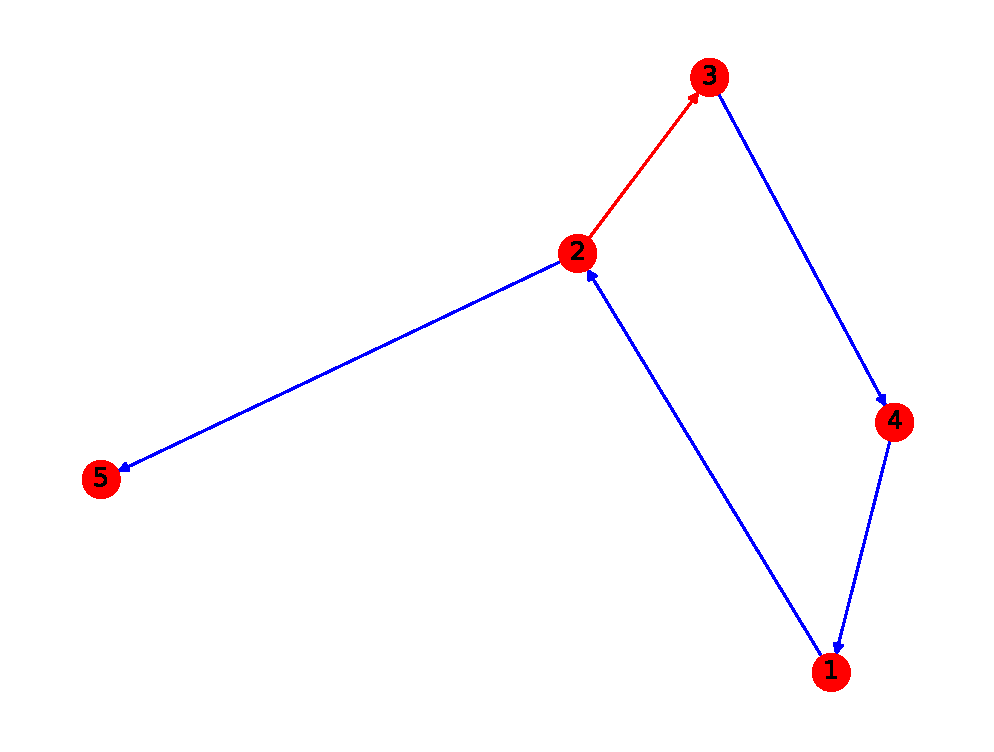
\includegraphics[width=\textwidth]{11-MDC}
    \caption{Multigrafo dirigido cíclico (los nodos 2 y 3 tienen múltiples aristas).}
    \label{fig:MDC}
\end{figure}


\subsection{Multigrafo dirigido reflexivo}
\begin{figure}[H]
    \includegraphics[width=\textwidth]{12-MDR}
    \caption{Multigrafo dirigido reflexivo (los nodos 3 y 4 tienen múltiples aristas, el nodo 1 tiene una arista reflexiva).}
    \label{fig:MDR}
\end{figure}


\section{Algoritmo \textit{Spring}}
Basado en la física, el algoritmo \textit{spring} trata de mantener que la suma de las fuerzas entre los nodos (los pesos de las aristas) sea de 0. Se basa esencialmente en la ley de Coulomb y en la métrica euclidiana para obtener estos valores, teniendo una complejidad computacional de $O(n^2)$ \cite{spring}.

\subsection{Grafo simple no dirigido reflexivo}
\begin{figure}[H]
    \includegraphics[width=\textwidth]{3-GSNDC}
    \caption{Grafo simple no dirigido reflexivo (el nodo 1 tiene una arista reflexiva).}
    \label{fig:GSNDR}
\end{figure}

\subsection{Grafo simple dirigido acíclico}
\begin{figure}[H]
    \includegraphics[width=\textwidth]{4-GSDA}
    \caption{Grafo simple dirigido acíclico}
    \label{fig:GSDA}
\end{figure}


\section{Algoritmo \textit{Shell}}
Similar al algoritmo circular, el algoritmo \textit{shell} realiza agrupaciones de nodos en círculos, con la diferencia que los nodos se pueden separar en distintos círculos a lo largo del grafo, por lo que la complejidad de este algoritmo es igual al algoritmo circular de $O(n)$ siendo $n$ el número de aristas \cite{shell}.


\subsection{Multigrafo no dirigido reflexivo}
\begin{figure}[H]
    \includegraphics[width=\textwidth]{9-MNDR}
    \caption{Multigrafo no dirigido reflexivo (los nodos 1 y 2 tienen múltiples aristas, el nodo 1 tiene una arista reflexiva).}
    \label{fig:MNDR}
\end{figure}

\section{Conclusiones entre algoritmos}
Los algoritmos estudiados tienen distintos propósitos, siendo el tipo de visualización que se desea del grafo para determinar el algoritmo más adecuado. Por ejemplo, para simples pruebas de visualización se utilizaría el algoritmo \textit{random} por su complejidad más simple entre los algoritmos, mientras que para otros tipos de grafos se utilizarían los otros tipos de algoritmos según el caso.

\bibliographystyle{plain}
\bibliography{references}

\end{document}
